% ============================================================
%  N.2.6  Eyeriss CS5: PE Array Aspect Ratio
% ============================================================
\subsection{Eyeriss: PE Array Aspect Ratio (CS5)}
\label{sec:eyeriss-cs5}

\subsubsection{Motivation}
Optimizing the PE array aspect ratio for EDP  (see Section\~\ref\{sec:cs4-aspect\}) is also essential in Eyeriss, because its spatial mapping distributes different loop dimensions across the two axes. Rows absorb weight-related factors (\$C\$, \$S\$, \$Z\$), whereas columns absorb output channel factors.

Therefore, a row-heavy array absorbs more weight factors spatially but forces larger channel residuals in the column direction, while a column-heavy configuration exhibits the inverse behavior. Ultimately, the optimal shape is governed by the relative size of the weight and activation dimensions in the fused workload.

To evaluate this trade-off, CS5 sweeps all power-of-two factorizations of a fixed PE budget (2,048 PEs for FSRCNN and MC-CNN; 16,384 PEs for VGG16 and ResNet18), tracking the resulting energy, latency, and EDP for every feasible mapping.


\subsubsection{Results}

\paragraph{ResNet18 (16\,384 PEs).}
Table~\ref{tab:eyeriss-cs5} lists the feasible configurations for
ResNet18, with a weight register size fixed.
Seven aspect ratios are feasible, from
$256 \times 64$ to the extreme row-heavy $16{,}384 \times 1$.
Latency is constant across all configurations, therefore the EDP ranking is determined entirely
by energy.
The best configuration is $256 \times 64$, and energy increases gently as
the array becomes more row-heavy.

The total variation is only $2.6\%$, indicating that for ResNet18 the
aspect ratio has a negligible impact once feasibility is achieved.

\begin{table}[htbp]
  \centering
  \caption{Eyeriss CS5: PE aspect ratio sweep for ResNet18
    (16\,384 total PEs, full fusion).
    Best EDP marked with~$\star$.}
  \label{tab:eyeriss-cs5}
  \begin{tabular}{lrrrr}
    \toprule
    Config & Rows & Cols & Energy ($\mu$J) & EDP (J$\cdot$cc) \\
    \midrule
    $256 \times 64$\,$\star$
           & 256   & 64  & $2.35 \times 10^{4}$ & $7.36 \times 10^{4}$ \\
    $512 \times 32$
           & 512   & 32  & $2.37 \times 10^{4}$ & $7.37 \times 10^{4}$ \\
    $1024 \times 16$
           & 1024  & 16  & $2.40 \times 10^{4}$ & $7.46 \times 10^{4}$ \\
    $2048 \times 8$
           & 2048  &  8  & $2.41 \times 10^{4}$ & $7.50 \times 10^{4}$ \\
    $4096 \times 4$
           & 4096  &  4  & $2.41 \times 10^{4}$ & $7.50 \times 10^{4}$ \\
    $8192 \times 2$
           & 8192  &  2  & $2.41 \times 10^{4}$ & $7.50 \times 10^{4}$ \\
    $16384 \times 1$
           &16384  &  1  & $2.41 \times 10^{4}$ & $7.50 \times 10^{4}$ \\
    \bottomrule
  \end{tabular}
\end{table}
The underlying reason is that ResNet18 features deep channel dimensions ($Z$ up to 512) that easily saturate a moderate column count. At 64~columns, the spatial mapping mechanism (\texttt{SACols}) effectively absorbs the most $Z$ factors. Conversely, if the array is constrained to fewer than 64~columns, the mapper is forced to handle the excess $Z$ dimensions temporally. This temporal folding increases the required capacity of the weight register to accommodate the larger residuals, which marginally raises the energy cost per access.

\paragraph{VGG16 (16\,384 PEs).}
Seven power-of-two factorizations from $256 \times 64$ to
$16{,}384 \times 1$ are feasible, all sharing the same latency.
The best EDP is $512 \times 32$, tied with $256 \times 64$.
Energy rises by $4.1\%$ at
$2{,}048 \times 8$ and plateaus thereafter, mirroring the ResNet18
behavior.

\paragraph{FSRCNN (2\,048 PEs).}
FSRCNN exhibits a broader feasibility range, with nine
power-of-two factorizations from $8 \times 256$ to $2{,}048 \times 1$
being feasible.
The best EDP is the most column-heavy configuration,
$8 \times 256$.
Energy is $5.7\%$ lower at $8 \times 256$ than at $64 \times 32$ and
beyond, where it plateaus.


\paragraph{MC-CNN (2\,048 PEs).}
Nine configurations are feasible from $8 \times 256$ to $2{,}048 \times 1$.
The best EDP is $128 \times 16$, tying with $256 \times 8$ through
$2{,}048 \times 1$, while $16 \times 128$ is within $0.2\%$
and offers the lowest latency among competitive configurations.
The most column-heavy configuration ($8 \times 256$) has higher latency because only 8 rows cannot absorb enough
weight factors spatially, forcing more temporal iterations.
MC-CNN therefore favors a moderate aspect ratio that balances row
absorption of weights with column distribution of channels.


\paragraph{Cross-workload comparison.}
Figure~\ref{fig:eyeriss-cs5} presents the energy (top row) and EDP
(bottom row) for all four workloads.
Two patterns emerge.
First, the weight-dominant workloads (VGG16, ResNet18) show nearly
flat energy and EDP curves across all seven feasible aspect ratios,
with total variation below $4.1\%$ for VGG16 and $2.6\%$ for
ResNet18.
Second, the activation-dominant workloads (FSRCNN, MC-CNN) display
a mild preference for column-heavy configurations, where the SACols
mechanism can distribute channel factors more effectively.
In all cases the EDP variation across feasible aspect ratios is
modest ($< 6\%$ for FSRCNN, $< 4.1\%$ for VGG16).

\begin{figure}[htbp]
  \centering
  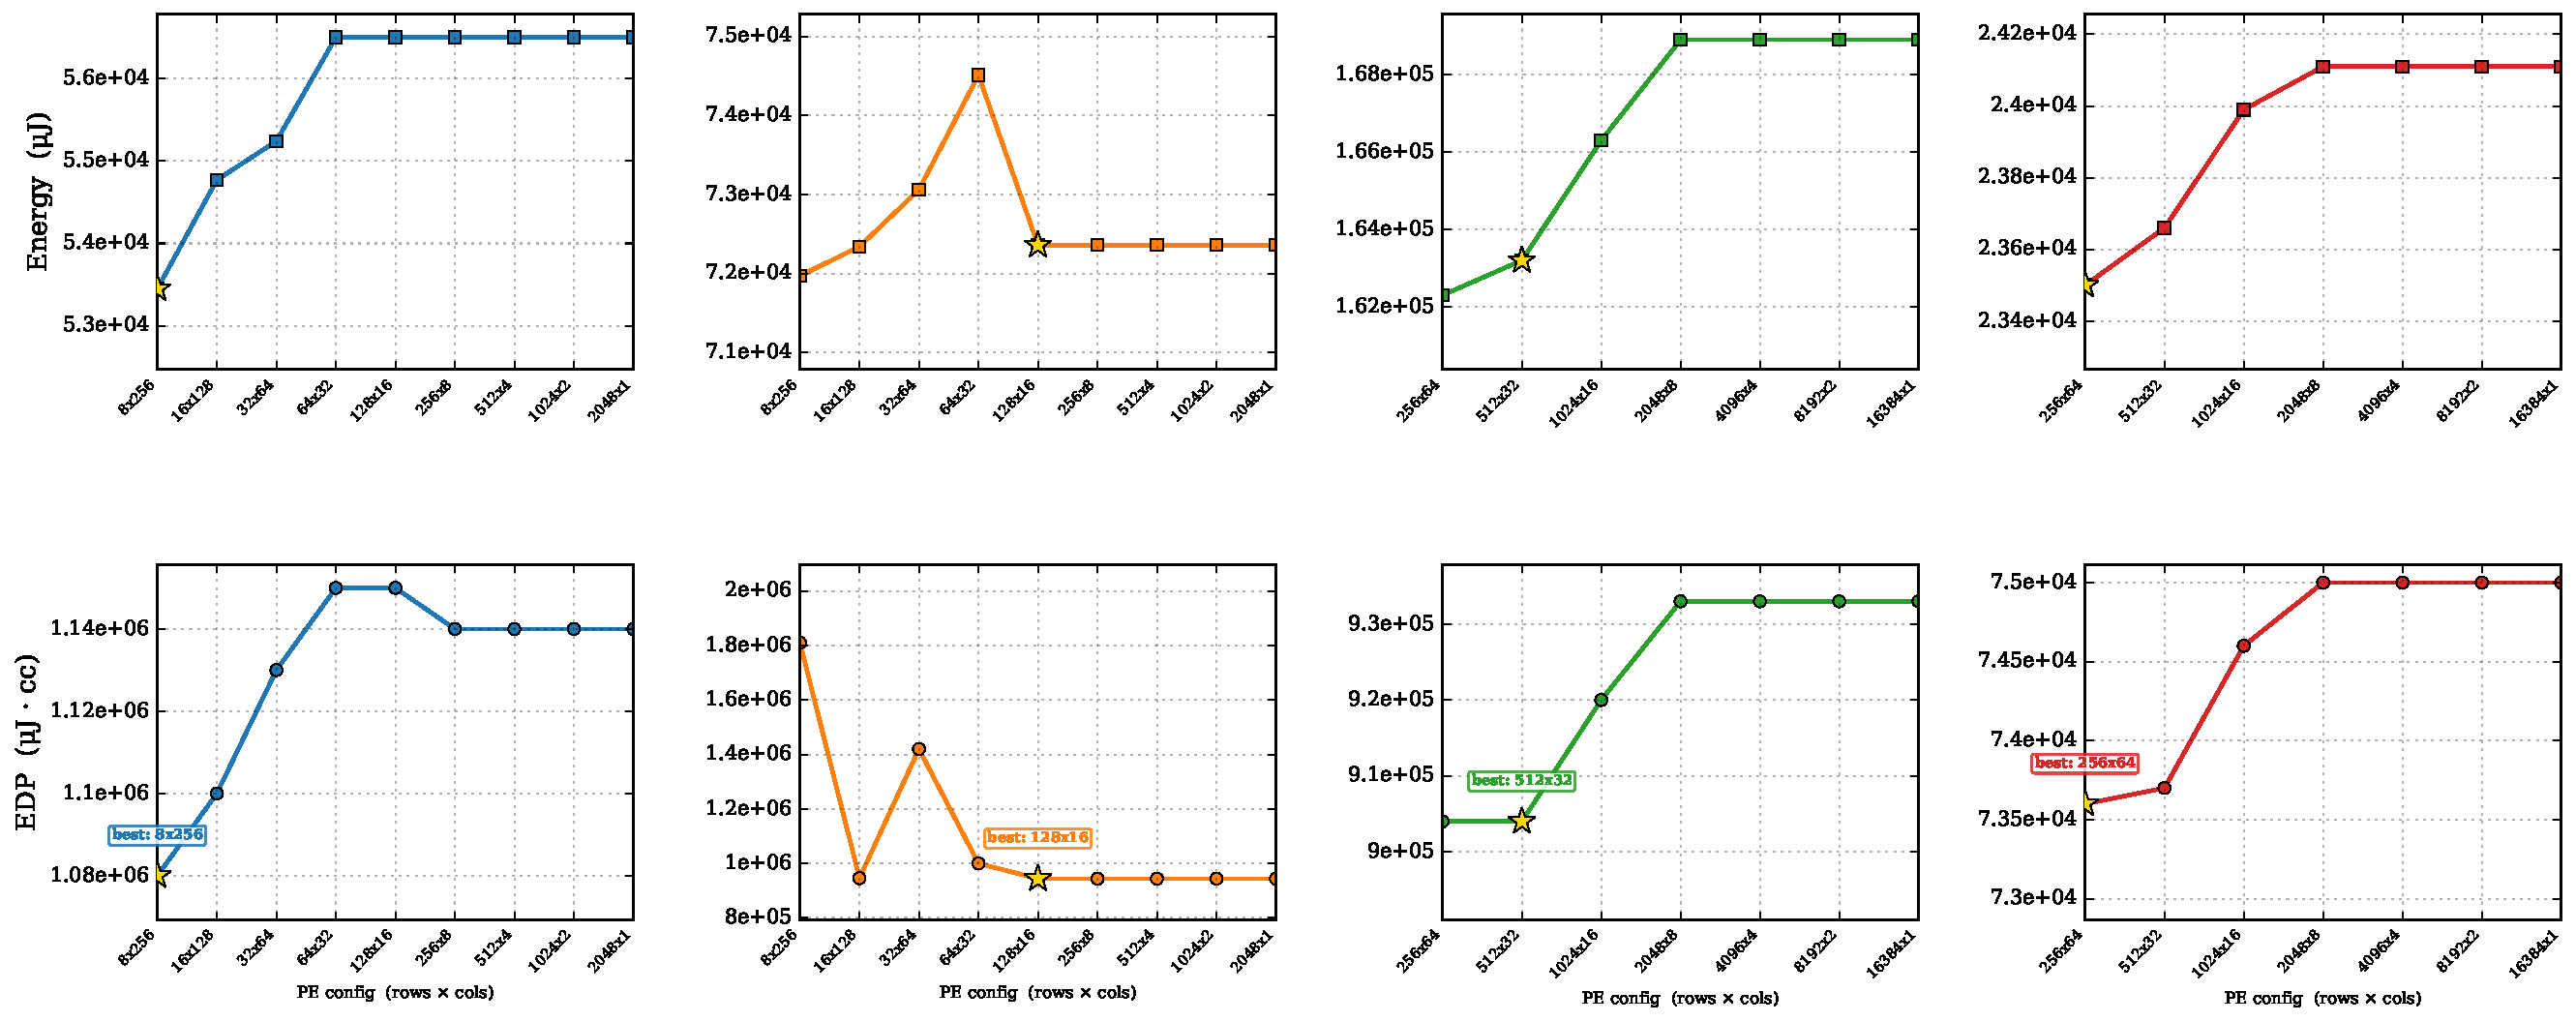
\includegraphics[width=0.95\textwidth]{plots/eyeriss_cs5_aspect_ratio.pdf}
  \caption{Eyeriss CS5: Energy (top) and EDP (bottom) vs.\ PE aspect
    ratio at fixed total PEs.
    Stars mark the best-EDP configuration for each workload.}
  \label{fig:eyeriss-cs5}
\end{figure}

\paragraph{Considerations}
Once the register sizes are set to satisfy the fused mapping
constraints, the PE aspect ratio has limited influence on energy and
EDP.
Column-heavy configurations offer a small advantage for workloads with
narrow channels, while weight-dominant workloads show nearly flat
curves regardless of aspect ratio once registers are adequately sized.